\section{Regressione Lineare}
In fisica, il moto uniforme è un tipo di moto in cui un oggetto si sposta con velocità costante. Questo significa che la distanza percorsa dall'oggetto è proporzionale al tempo impiegato. La relazione tra spazio \( y \) e tempo \( x \) in un moto uniforme può essere espressa tramite la seguente equazione lineare:

\[
y = v \cdot x + s_0
\]

dove:
\begin{itemize}
    \item \( v \) è la velocità costante dell'oggetto (pendenza della retta).
    \item \( s_0 \) è la posizione iniziale dell'oggetto (intercetta della retta).
\end{itemize}

L'obiettivo è trovare i parametri \( v \) e \( s_0 \) che meglio rappresentano i dati sperimentali. Utilizzando una regressione lineare, possiamo ottenere questi parametri adattando una retta ai dati.

\subsection{Tabella dei Dati}

Per l'analisi, consideriamo i seguenti dati sperimentali raccolti per tempo e spazio:

\begin{table}[h!]
    \centering
    \begin{tabular}{|c|c|}
    \hline
    \textbf{Tempo (\si{\second})} & \textbf{Spazio (\si{\meter})} \\
    \hline
    1.0 & 2.0 \\
    2.0 & 4.0 \\
    3.0 & 6.0 \\
    4.0 & 8.0 \\
    5.0 & 10.0 \\
    \hline
    \end{tabular}
    \caption{Dati sperimentali di tempo e spazio.}
    \label{tab:dati}
\end{table}

\subsection{Regressione Lineare}

La regressione lineare cerca di adattare una retta ai dati sperimentali, trovando i parametri \( a \) e \( b \) che minimizzano la somma dei quadrati delle differenze tra i valori osservati e quelli previsti dalla retta. In questo caso, la retta di regressione è data da:

\[
y = a \cdot x + b
\]

dove:
\begin{itemize}
    \item \( a \) è la pendenza della retta, che rappresenta la velocità \( v \).
    \item \( b \) è l'intercetta, che rappresenta la posizione iniziale \( s_0 \).
\end{itemize}

\subsection{Uso di Python per la Regressione Lineare}
Per calcolare i parametri della retta di regressione e il loro errore, utilizziamo il modulo \texttt{scipy.optimize.curve\_fit} di Python, che permette di adattare una funzione ai dati sperimentali. La funzione \texttt{curve\_fit} ritorna i parametri ottimizzati e le loro deviazioni standard. Utilizziamo anche \texttt{matplotlib} per visualizzare i dati e la retta di regressione.


Ecco il codice Python utilizzato:

\begin{lstlisting}[caption={Semplice regressione lineare}]
import numpy as np
from scipy.optimize import curve_fit
import matplotlib.pyplot as plt
# Dati sperimentali
tempo = np.array([1.0, 2.0, 3.0, 4.0, 5.0])
spazio = np.array([1.9, 4.1, 6.0, 7.7, 12.0])

# Definizione della funzione di modello lineare
def linear_model(x, a, b):
    return a * x + b

# Fitting dei dati
params, params_covariance = curve_fit(linear_model, tempo, spazio)

# Estrazione dei parametri
pendenza, intercetta = params
pendenza_error, intercetta_error = np.sqrt(np.diag(params_covariance))

print(f"Pendenza: {pendenza:.3f} +- {pendenza_error:.3f}")
print(f"Intercetta: {intercetta:.3f} +- {intercetta_error:.3f}")

# Creazione del grafico
plt.figure(figsize=(8, 6))
plt.scatter(tempo, spazio, label='Dati sperimentali')
plt.plot(tempo, linear_model(tempo, *params), 'r-', label='Retta di regressione')
plt.xlabel('Tempo (s)')
plt.ylabel('Spazio (m)')
plt.title('Fitting Lineare')
plt.legend()
plt.grid(True)
plt.savefig('regressione_lineare.png')  # Salvataggio dell'immagine
#se vuoi scaricare il file da google colab decommenta le righe:
#from google.colab import files
#files.download('regressione_lineare.png')
plt.show()
\end{lstlisting}

\subsection{Output del Codice Python}

L'output del codice Python è il seguente:

\begin{mdframed}[backgroundcolor=lightgray, linecolor=black, linewidth=1pt]
\textbf{Pendenza}: \(2.020 \pm 0.083 \, \si{\meter\per\second}\) \\
\textbf{Intercetta}: \(0.200 \pm 0.276 \, \si{\meter}\)
\end{mdframed}

\textbf{Pendenza}: La pendenza della retta di regressione è \(2.020 \pm 0.083 \, \si{\meter\per\second}\). Questo valore rappresenta la velocità media del moto. L'errore associato indica l'incertezza nella determinazione della pendenza, che riflette la variabilità dei dati sperimentali rispetto alla retta di regressione.

\textbf{Intercetta}: L'intercetta della retta di regressione è \(0.200 \pm 0.276 \, \si{\meter}\). Questo valore rappresenta la posizione iniziale, cioè il valore di \(y\) quando \(x\) è zero. L'errore associato all'intercetta indica l'incertezza nella misura del punto in cui la retta di regressione interseca l'asse delle ordinate. Questo valore può dare indicazioni sul punto di partenza del movimento descritto dai dati.



Di seguito , in figura \ref{fig:regressione_lineare} è mostrato il grafico della regressione lineare che visualizza i dati sperimentali insieme alla retta di regressione ottenuta.

\begin{figure}[h!]
    \centering
    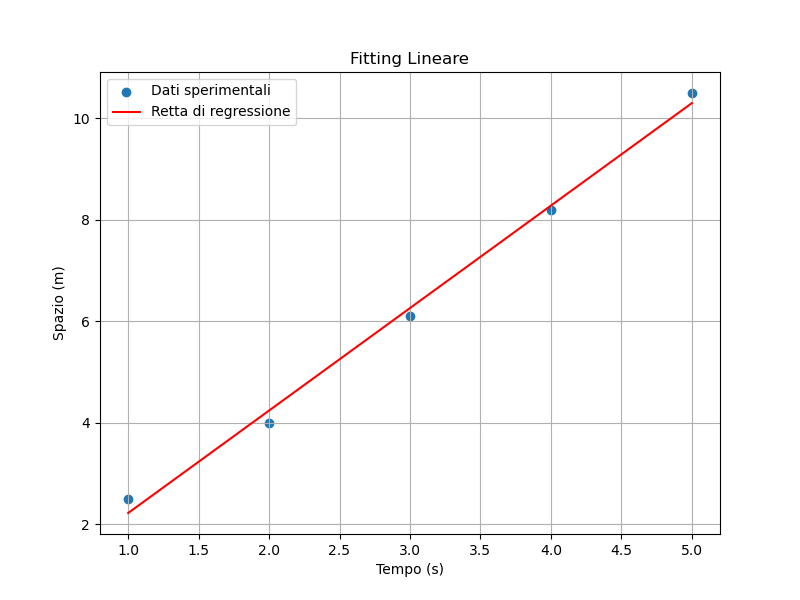
\includegraphics[width=0.8\textwidth]{regressione_lineare.png}
    \caption{Grafico della regressione lineare: i dati sperimentali sono mostrati come punti, e la retta di regressione è mostrata in rosso.}
    \label{fig:regressione_lineare}
\end{figure}


